%%=============================================================================
%% Case Study
%%=============================================================================

\chapter{Case study}%
\label{ch:casestudy}

\section{Introduction}%
\label{sec:introduction-casestudy}
This chapter will include the best practices and clean-up methods performed on the CI/CD pipeline at Wolters Kluwer and the metrics and results that were obtained from the clean-up. The chapter will include the CPU utilization, memory usage, build metrics, resource utilization, and system uptime of the CI/CD pipeline.

\section{Best Practices}%
\label{sec:best-practices}
The case study at Wolters Kluwer involved the implementation of best practices to improve the CI/CD pipeline. In following subsections the best practices are discussed.

\subsection{Remove build configuration with wrong Version Control System}%
\label{sub:remove-build-configuration-with-wrong-version-control-system}
The first best practice that was implemented was the removal of build configurations with the wrong version control system. This was done to ensure that the CI/CD pipeline was not cluttered with unnecessary build configurations. The removal of these build configurations helped to improve the efficiency and performance of the CI/CD pipeline.

\subsection{Detect build configurations with simultaneous running builds}%
\label{sub:detect-build-configurations-with-simultaneous-running-builds}
The second best practice that was implemented was the detection of build configurations with simultaneous running builds. This was done to identify build configurations that were running simultaneously and to ensure that the CI/CD pipeline was not overloaded. Simultaneous runnign builds can take a lot of resources and can slow down the CI/CD pipeline.

\subsection{Remove build configurations with no recent builds}%
\label{sub:remove-build-configurations-with-no-recent-builds}
Build configurations with no recent builds were archived or removed. This would help to reduce the clutter in the CI/CD pipeline and improve the performance of the pipeline.

\subsection{Remove artifacts of archived build configurations}%
\label{sub:remove-artifacts-of-archived-build-configurations}
Artifacts can take up a lot of space and those of archived build configurations are not needed anymore. This could free up a lot of space and improve the performance of the CI/CD pipeline.

\subsection{Automation of build agents}%
\label{sub:automation-of-build-agents}
By automating build agents, the CI/CD pipeline can be scaled up or down based on the demand. This would help to improve the scalability and usage of the CI/CD pipeline.

\subsection{Windows vs Linux}%
\label{sub:windows-vs-linux}
It was difficult to test this best practice. Wolters Kluwer uses build agents that run on Windows and Linux. Powershell script are easier to run on Windows and bash scripts are easier to run on Linux.


\section{CPU Utilization}%
\label{sec:cpu-utilization}

The CPU utilization is shown in figure \ref{fig:cpu}. The time range goes from the beginning of the case study at Wolters Kluwer untill the end. The clean up of the CI/CD environment hasn't reduced the CPU utilization clearly.

\begin{figure}[htbp]
    \centering
    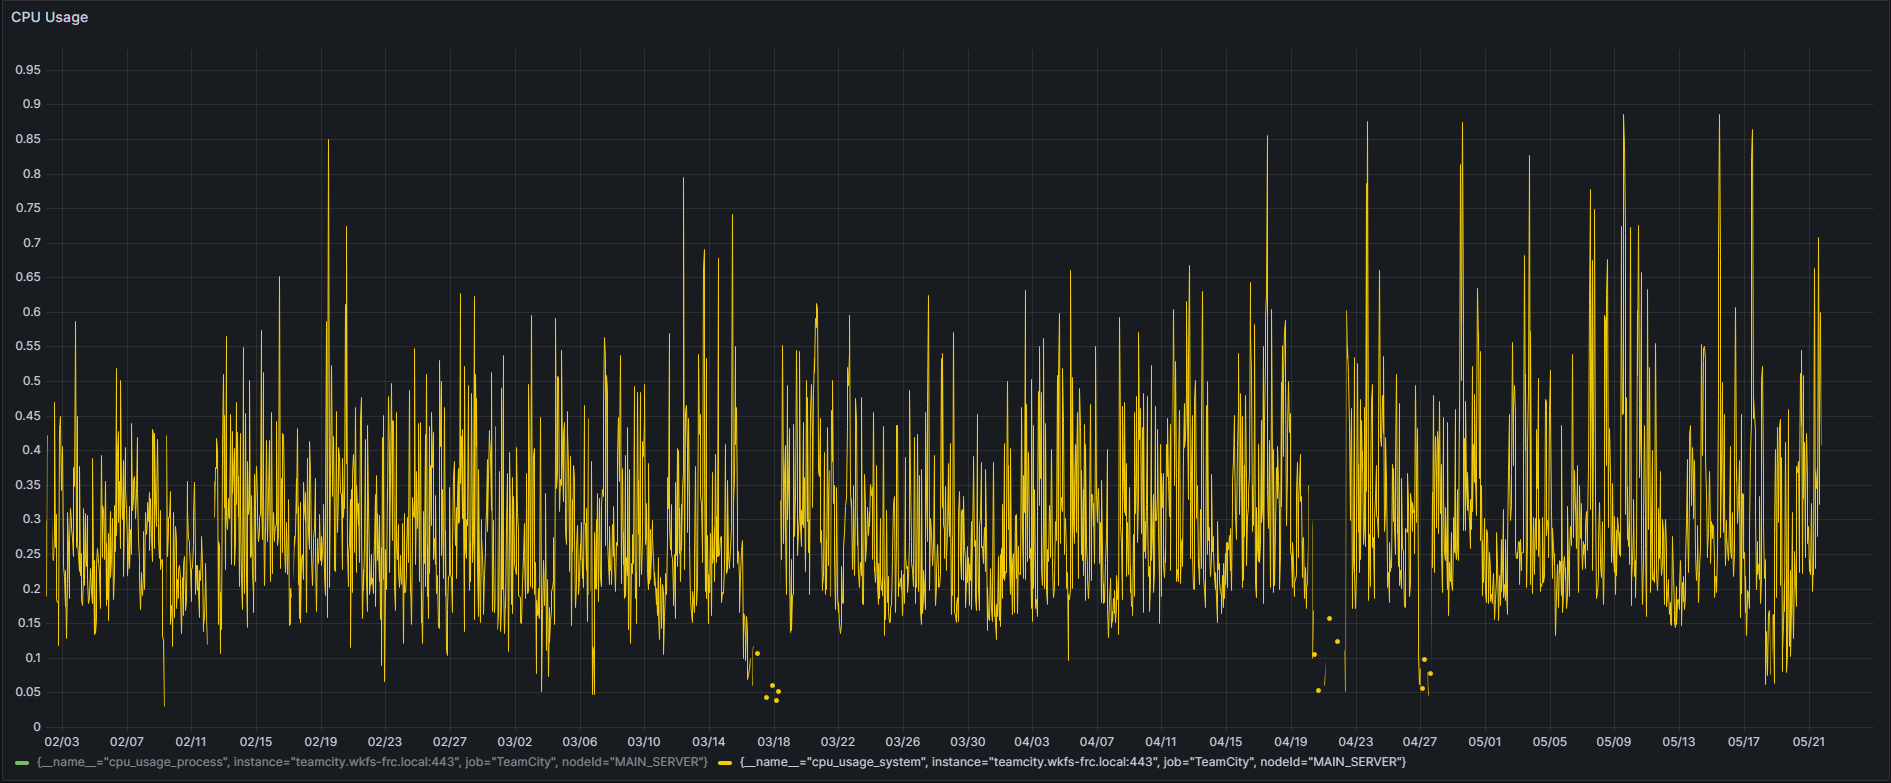
\includegraphics[width=\textwidth]{graphics/cpu.png}
    \caption{CPU Usage}
    \label{fig:cpu}
\end{figure}

\section{Memory Usage}%
\label{sec:memory-usage}

The memory usage is shown in figure \ref{fig:memory}. The green line represents the memory usage of the Eden Space. In the Eden Space new objects are allocated. The yellow line represents the memory usage of the Old Gen, it is where long living objects are stored. We can see a decrease especially in the Old Gen memory usage. 

\begin{figure}[htbp]
    \centering
    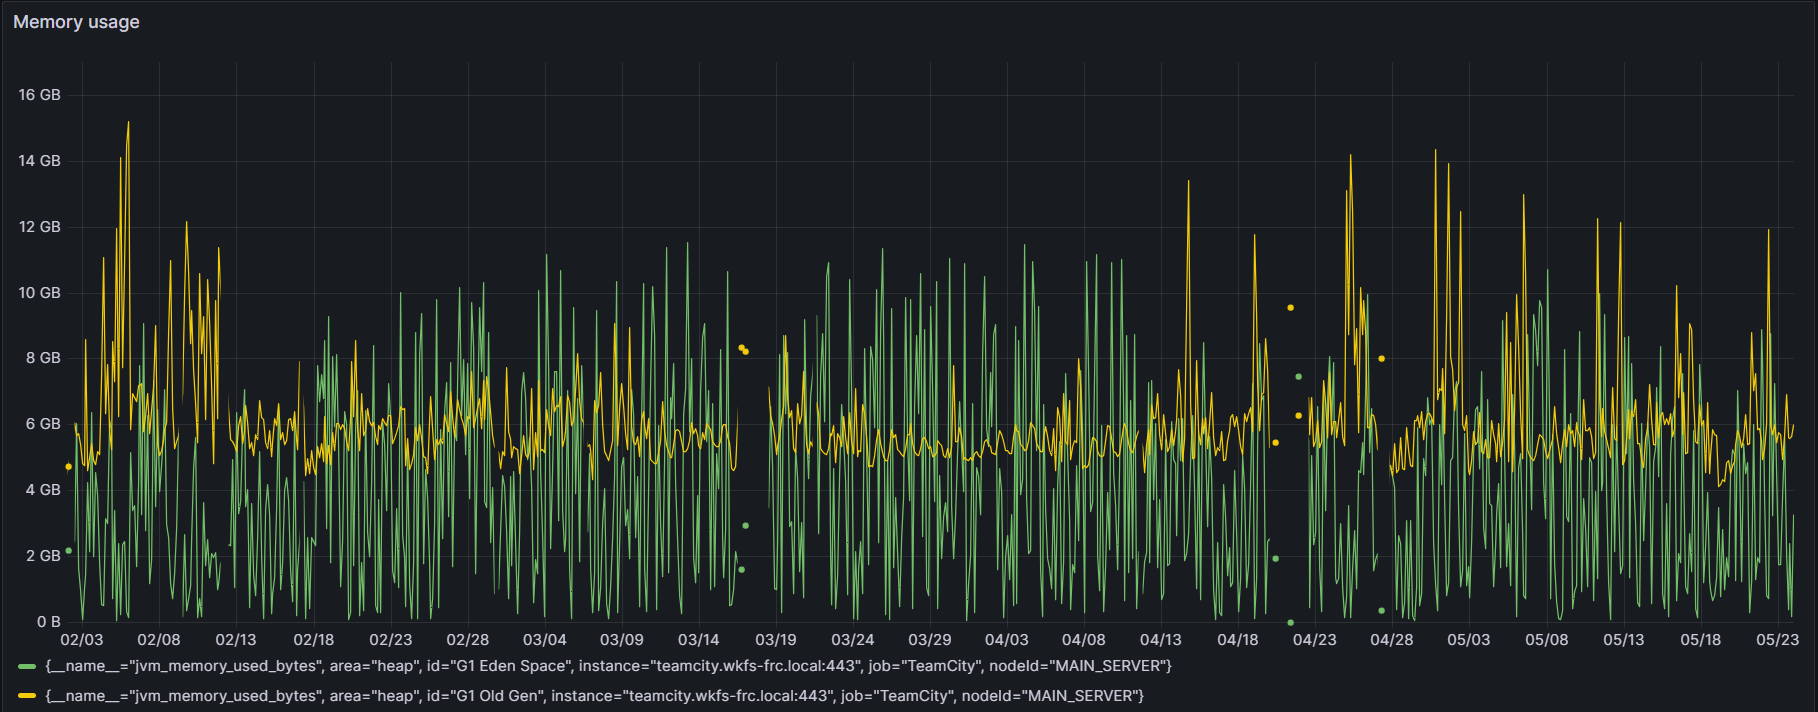
\includegraphics[width=\textwidth]{graphics/memory.png}
    \caption{Memory Usage}
    \label{fig:memory}
\end{figure}

\section{Build Metrics}%
\label{sec:build-metrics}

The amount of builds running at the same time is shown in figure \ref{fig:builds}. There isn't that much difference in the amount of builds running at the same time.

\begin{figure}[htbp]
    \centering
    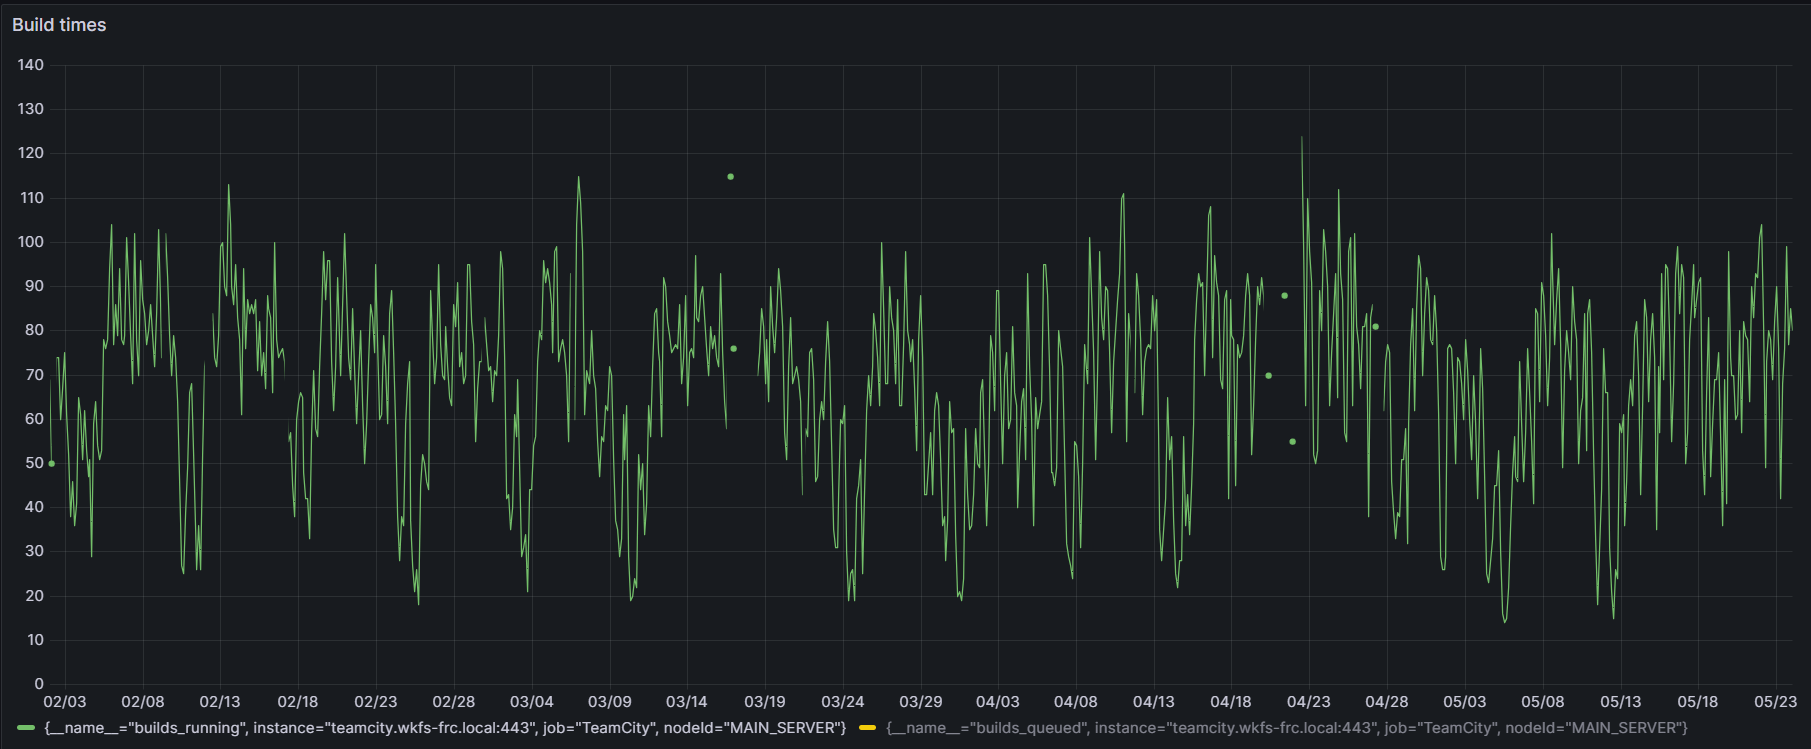
\includegraphics[width=\textwidth]{graphics/builds running.png}
    \caption{Builds running at the same time}
    \label{fig:builds-running}
\end{figure}

The amount of queued builds at the same time is shown in figure \ref{fig:queued-builds}. The average decreased a little bit but there are still some peaks.

\begin{figure}[htbp]
    \centering
    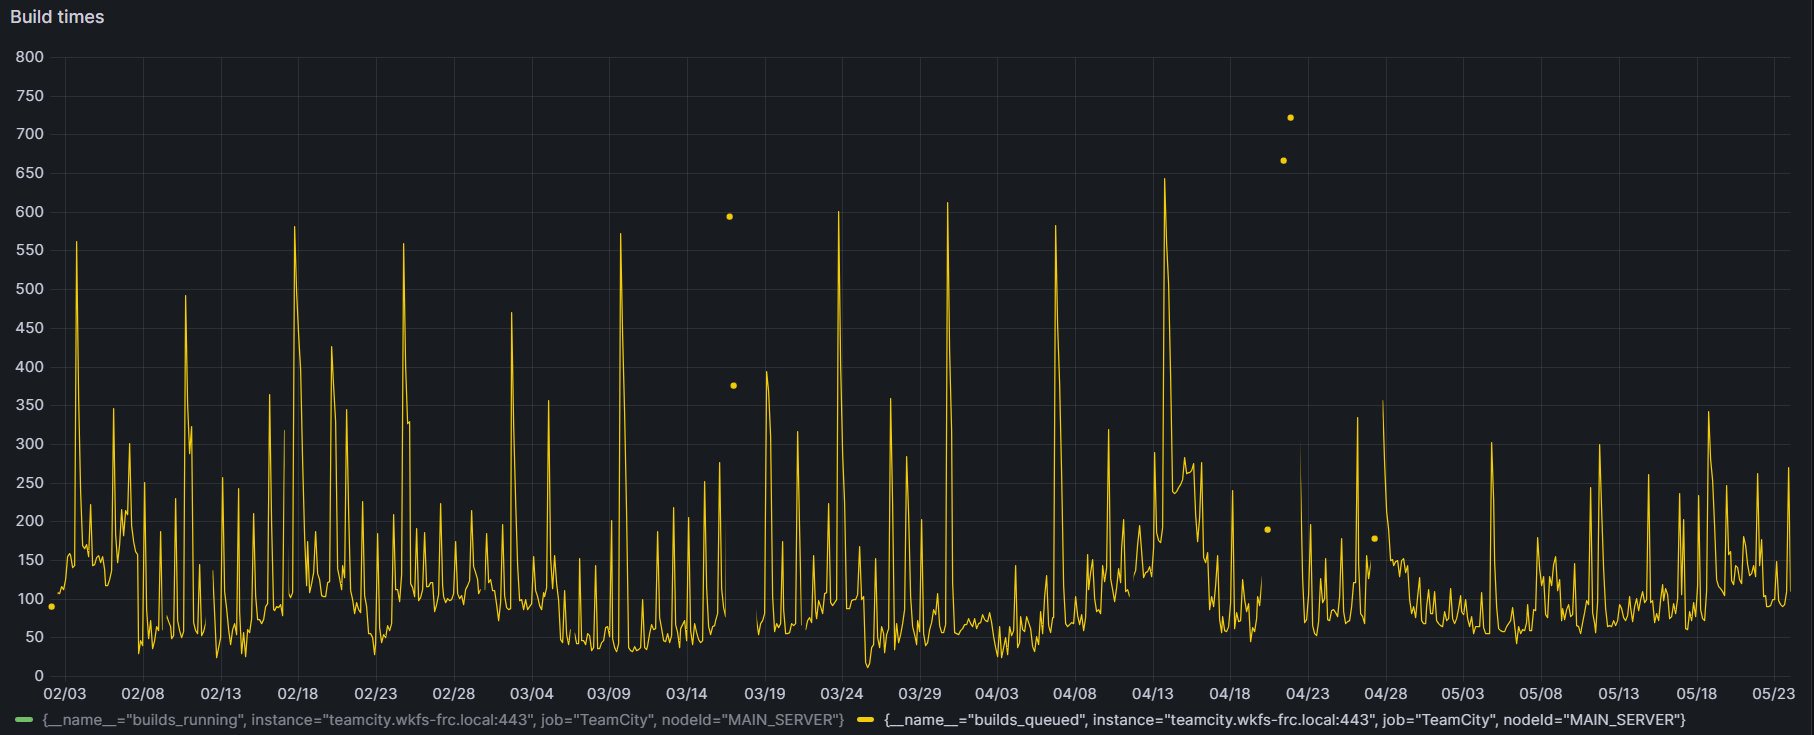
\includegraphics[width=\textwidth]{graphics/builds queued.png}
    \caption{Queued builds}
    \label{fig:queued-builds}
\end{figure}

\section{Resource Utilization}%
\label{sec:resource-utilization}

